% !TEX root = mythesis.tex

%==============================================================================
\chapter{Mesonic Signal Saturation}
\label{sec:signal}
%==============================================================================
% \newcommand{\todo}[1]{\textbf{\color{red}TODO: #1}}
The meson mass spectrum is extracted via Bayesian analysis of two-point correlation functions. One can systematically improve the agreement with PDG values by using more statistics, employing a collection of ensembles with various quark mass values and lattice spacing. Ultimately, the continuum masses are what we are after.
We perform a study of the resulting mesonic correlator signal using various distillation parameters to determine the optimal parameters to use. In particular, we want to test the optimal size of the eigenvector basis used to generate our perambulators and elementals, as well as the number of source locations per configuration in order to obtain a good signal while keeping the computational cost contained. 

% $(\bar{\psi}^{f_1}(n)\Gamma\psi^{f_2}(n))^{\dagger} = \pm \bar{\psi}^{f_2} \Gamma \psi^{f_1}$
% which can be derived from the fact that the interchange of Grassmann variables induces a minus sign and the $\gamma_4$ appears via the relation $\bar{\psi} = \psi^{\dagger}\gamma_4$ \cite{Gattringer2009QuantumCO}. The conjugate interpolator is obtained by interchanging the $\psi$ and $\bar{\psi}$ and ordering the barred quark fields to the left. 

% Now we actually have to evaluate the correlators by employing the property that the fermionic expectation value factorizes with respect to the flavors. We then apply wick's theorem for each of the two flavors, this is fermion contraction, by which we obtain the Dirac operators. In this case, only Grassmann variables with equal flavor can be contracted with each other.

Given an operator with pion quantum numbers, such as
\[
\phi_L(x) = \bar{d}(x)\gamma_5u(x)
\]
or some smeared version of this, denoted $\phi_S(x)$,
the dimensionless correlator from Euclidean time $t_i$ to Euclidean time $t_f$
with momentum $\vec p$ is
\begin{eqnarray}
\Gamma^{\pi\pi}_{AB}(t_i,t_f,\vec{p})
 &=& a^6\sum_{{\vec x}_f}e^{-i(\vec{x}_f-\vec{x}_i)\cdot\vec{p}}
     \left<0\left|\phi_B(x_f)\phi_A^\dagger(x_i)\right|0\right> \nonumber \\
\end{eqnarray}


Here we present results for a systematic study of how the signal of the pion two-point correlator with $\vec{p}=(0,0,0)$ at zero displacement is affected by the rank of the distillation basis (number of eigenvectors used $n_{\text{vec}}$) and the number of $t_{src}$ insertions. The rank of the distillation basis take values in the set $n_{vec}\in {32,64,96,128}$ and the number of $t_{src} \in {1,2,4,8,12,24}$. We perform this study on the ensemble $\beta = 3.7$, $m_{ud}=-0.0220$, $m_s = -0.0$, $L^3 \times T = 32^3\times96$. This determination will allow us to optimize compute resources for the eigenbasis, perambulators, and elementals for the rest of the ensembles we have generated. We chose the pion as a test case as it typically provies the cleanest signal in lattice calculations. With this complete, we will proceed with computing the fundamental distillation objects using a distillation basis of rank 96 and 24 $t_{src}$ insertions for the perambulators.  

% \begin{figure}[h]
% 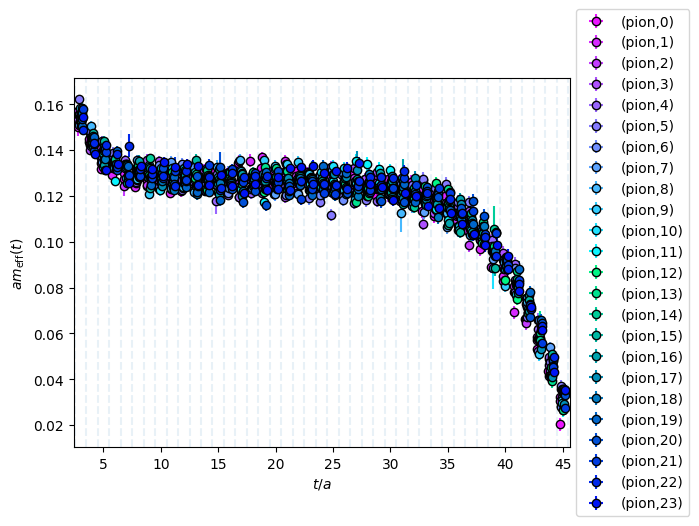
\includegraphics[width=0.75\textwidth]{eff.png}
% \caption{Effective mass plot of pion correlators for each $t_{tsrc}$ insertion after shifting all to the origin}
% \label{fig:figure10}
% \end{figure}
% \begin{figure}[h]
%     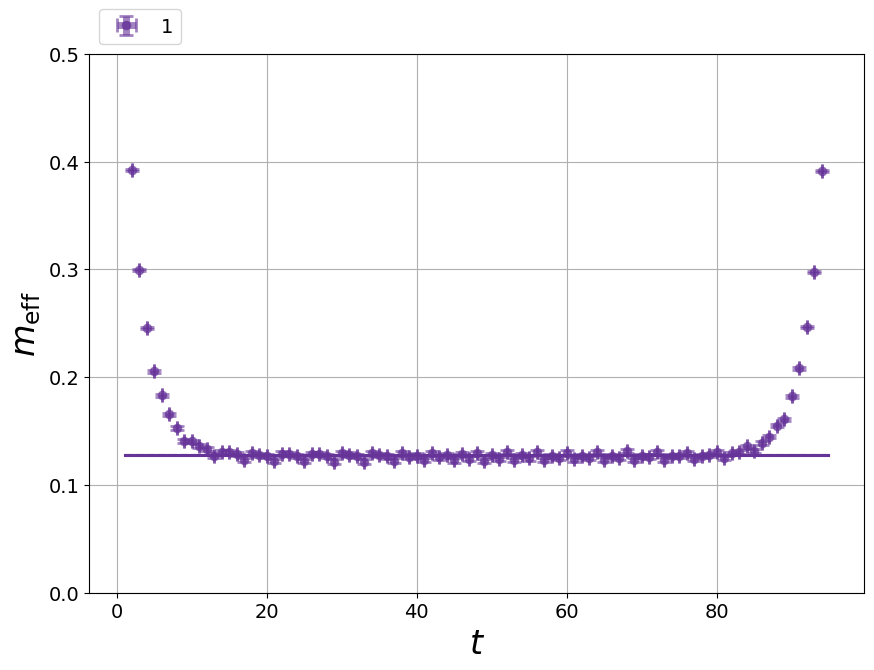
\includegraphics[width=0.8\textwidth]{nskip_1.png}
%     \caption{single state fit to the effective mass of the pion for 24 $t_{src}$ insertions}
%     \label{fig:figure4}
%     \end{figure}

% \begin{figure}[h]
% 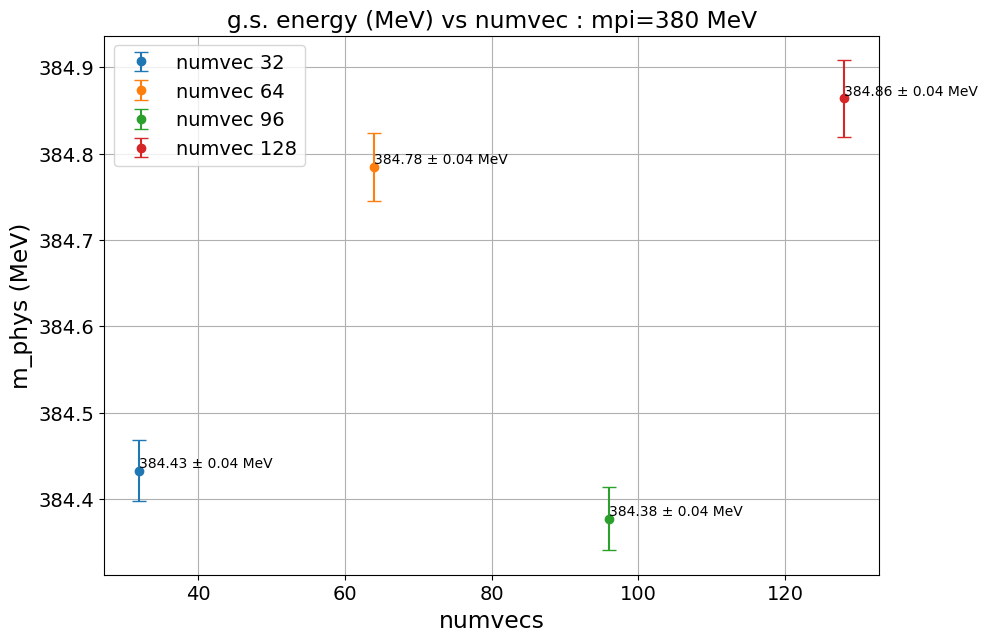
\includegraphics[width=0.8\textwidth]{nvecs.png}
% \caption{comparison of ground state energy of the pion for different sizes(rank) of the distillation basis}
% \label{fig:figure2}
% \end{figure}
% \begin{figure}[h]
% 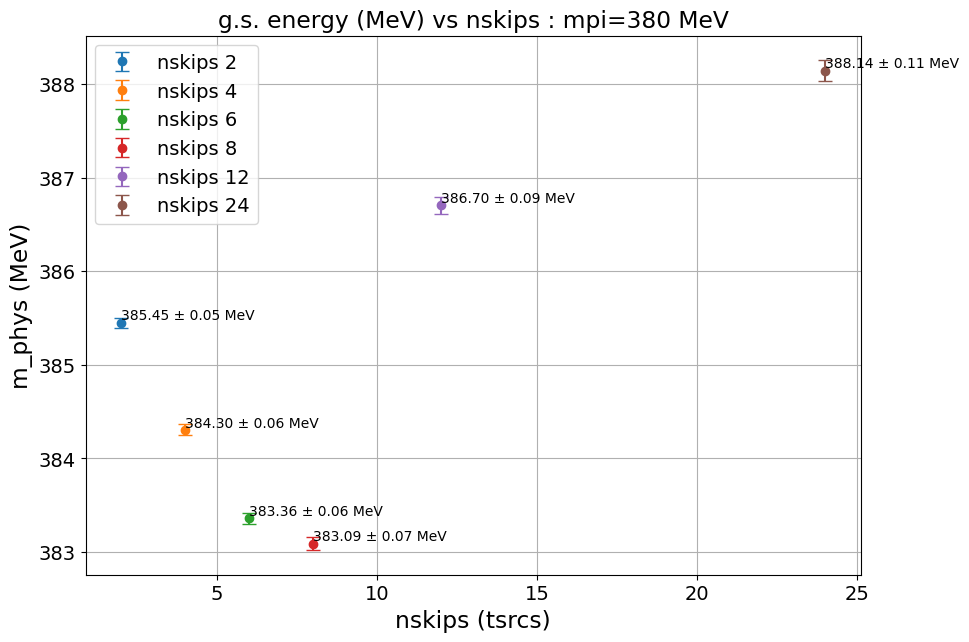
\includegraphics[width=0.8\textwidth]{tsrc_nskips.png}
% \caption{comparison of ground state energy of the pion for various number of $t_{src}$ insertions}
% \label{fig:figure3}
% \end{figure}

\begin{figure}[h]
    \centering
    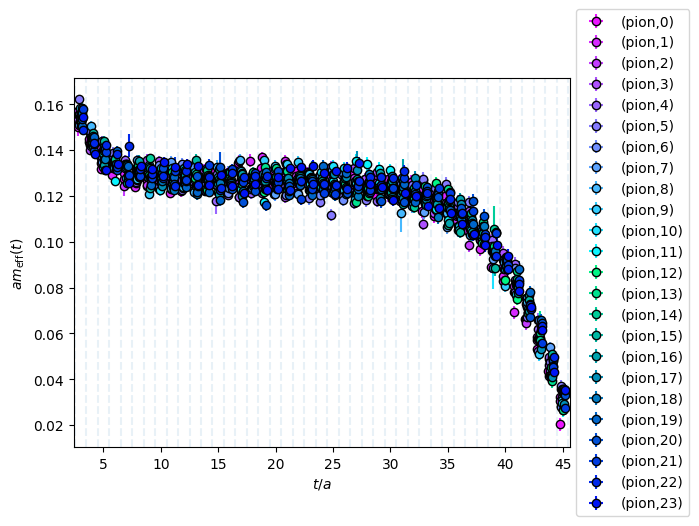
\includegraphics[width=0.9\textwidth]{eff.png}
    \caption{Effective mass plot of pion correlators for each $t_{tsrc}$ insertion after shifting all to the origin.}
    \label{fig:figure10}
\end{figure}

\begin{figure}[h]
    \centering
    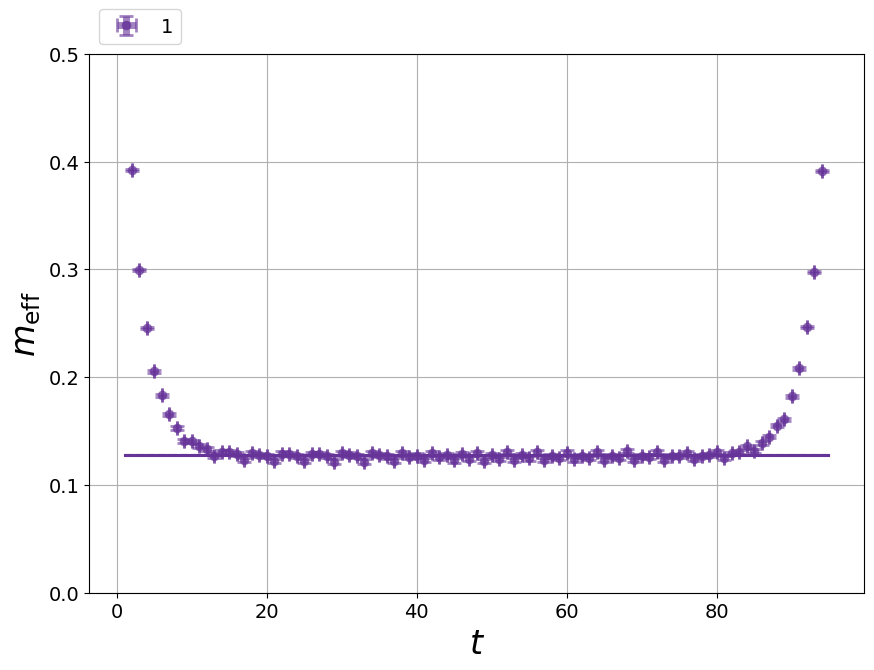
\includegraphics[width=0.9\textwidth]{nskip_1.png}
    \caption{Single state fit to the effective mass of the pion for 24 $t_{src}$ insertions.}
    \label{fig:figure4}
\end{figure}

\newpage

\begin{figure}[h]
    \centering
    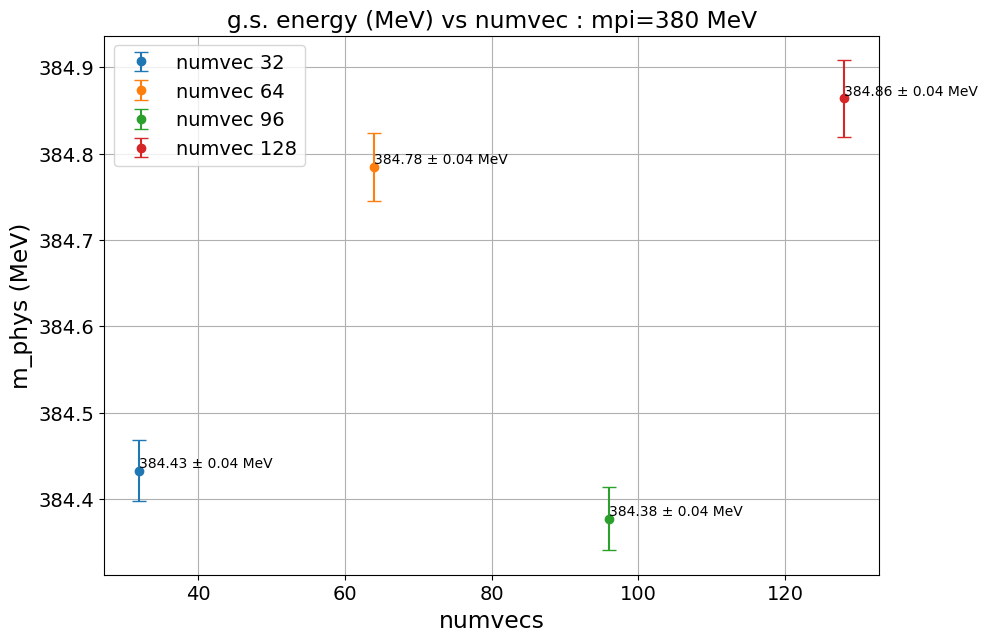
\includegraphics[width=0.9\textwidth]{nvecs.png}
    \caption{Comparison of ground state energy of the pion for different sizes (rank) of the distillation basis.}
    \label{fig:figure2}
\end{figure}

\begin{figure}[h]
    \centering
    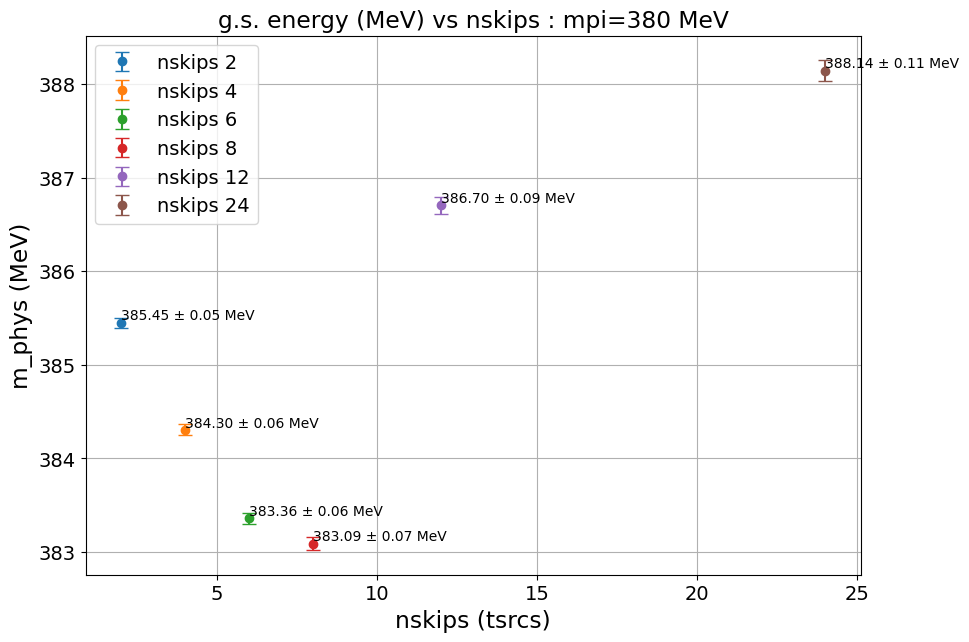
\includegraphics[width=0.9\textwidth]{tsrc_nskips.png}
    \caption{Comparison of ground state energy of the pion for various numbers of $t_{src}$ insertions.}
    \label{fig:figure3}
\end{figure}


